% Adjust these for the path of the theme and its graphics, relative to this file
%\usepackage{beamerthemeFalmouthGamesAcademy}
\usepackage{../../beamerthemeFalmouthGamesAcademy}
\usepackage{multimedia}
\graphicspath{ {../../} }

% Default language for code listings
\lstset{language=C++,
        morekeywords={each,in,nullptr}
}

% For strikethrough effect
\usepackage[normalem]{ulem}
\usepackage{wasysym}

\usepackage{pdfpages}

% http://www.texample.net/tikz/examples/state-machine/
\usetikzlibrary{arrows,automata}

\begin{document}
\title{Finite State Machines}
\subtitle{COMP110: Principles of Computing}

\frame{\titlepage} 

\part{Finite state machines}
\frame{\partpage}

\begin{frame}{Finite state machines}
    \begin{itemize}
        \item A \textbf{finite state machine (FSM)} consists of: \pause
            \begin{itemize}
                \item A set of \textbf{states}; and \pause
                \item \textbf{Transitions} between states \pause
            \end{itemize}
        \item At any given time, the FSM is in a \textbf{single state} \pause
        \item \textbf{Inputs} or \textbf{events} can cause the FSM to transition to a different state
    \end{itemize}
\end{frame}

\begin{frame}{State transition diagrams}
    \begin{center}\scalebox{0.8}{
        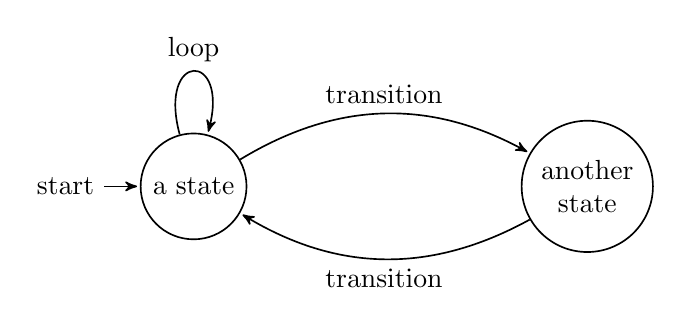
\begin{tikzpicture}[->,>=stealth',shorten >=1pt,auto,node distance=5cm,
                            semithick]
            \node[initial,state] (A) {a state};
            \node[state] (B) [right of=A, align=center] {another\\state};

            \path (A) edge [bend left] node [above] {transition} (B)
                  (B) edge [bend left] node [below] {transition} (A)
                  (A) edge [loop above] node {loop} (A);
        \end{tikzpicture}
    }\end{center}
    \begin{itemize}
        \item FSMs are often drawn as \textbf{state transition diagrams}
        \item Reminiscent of \textbf{flowcharts} and certain types of \textbf{UML diagram} \pause
    \end{itemize}
\end{frame}

\begin{frame}{FSMs for AI behaviour}
    The next slide shows a simple FSM for the following AI behaviour, for an enemy NPC in a shooter game: \pause
    \begin{itemize}
        \item By default, patrol (e.g.\ along a preset route) \pause
        \item If the player is spotted, attack them \pause
        \item If the player is no longer visible, resume patrolling \pause
        \item If you are low on health, run away and find a medikit. Then resume patrolling \pause
        \item If you are low on ammo, run away and find ammo. Then resume patrolling \pause
    \end{itemize}
\end{frame}

\begin{frame}
    \begin{center}\scalebox{0.8}{
        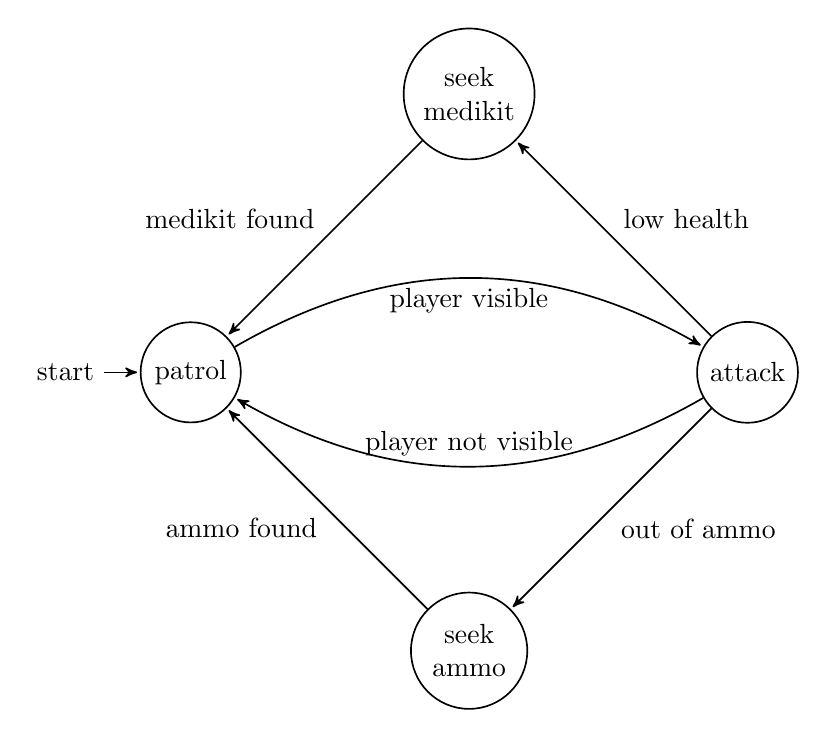
\begin{tikzpicture}[->,>=stealth',shorten >=1pt,auto,node distance=5cm,
                            semithick]
            \node[initial,state] (patrol) {patrol};
            \node[state] (health) [above right of=patrol, align=center] {seek\\medikit};
            \node[state] (ammo) [below right of=patrol, align=center] {seek\\ammo};
            \node[state] (attack) [above right of=ammo] {attack};

            \path (patrol) edge [bend left] node [below] {player visible} (attack)
                  (attack) edge [bend left] node [above] {player not visible} (patrol)
                  (attack) edge node [above right] {low health} (health)
                  (attack) edge node {out of ammo} (ammo)
                  (health) edge node [above left] {medikit found} (patrol)
                  (ammo) edge node {ammo found} (patrol);
        \end{tikzpicture}
    }\end{center}
\end{frame}

\begin{frame}{Other uses of FSMs}
    As well as AI behaviours, FSMs may also be used for: \pause
    \begin{itemize}
        \item Animation \pause
        \item UI menu systems \pause
        \item Dialogue trees \pause
        \item Token parsing \pause
        \item ...
    \end{itemize}
\end{frame}

\begin{frame}{Beyond FSMs}
    Some topics for you to research, for when plain old FSMs aren't enough... \pause
    \begin{itemize}
        \item Hierarchical FSMs
        \item Nested FSMs
        \item Stack-based FSMs
        \item Hierarchical task networks
        \item ...
    \end{itemize}
		Plus the topic we will be looking at today: \textbf{behaviour trees}
\end{frame}


% -------------------------------------------------------

%\part{The compiler}
%\frame{\partpage}
%
%\begin{frame}
%	\frametitle{The build process}
%	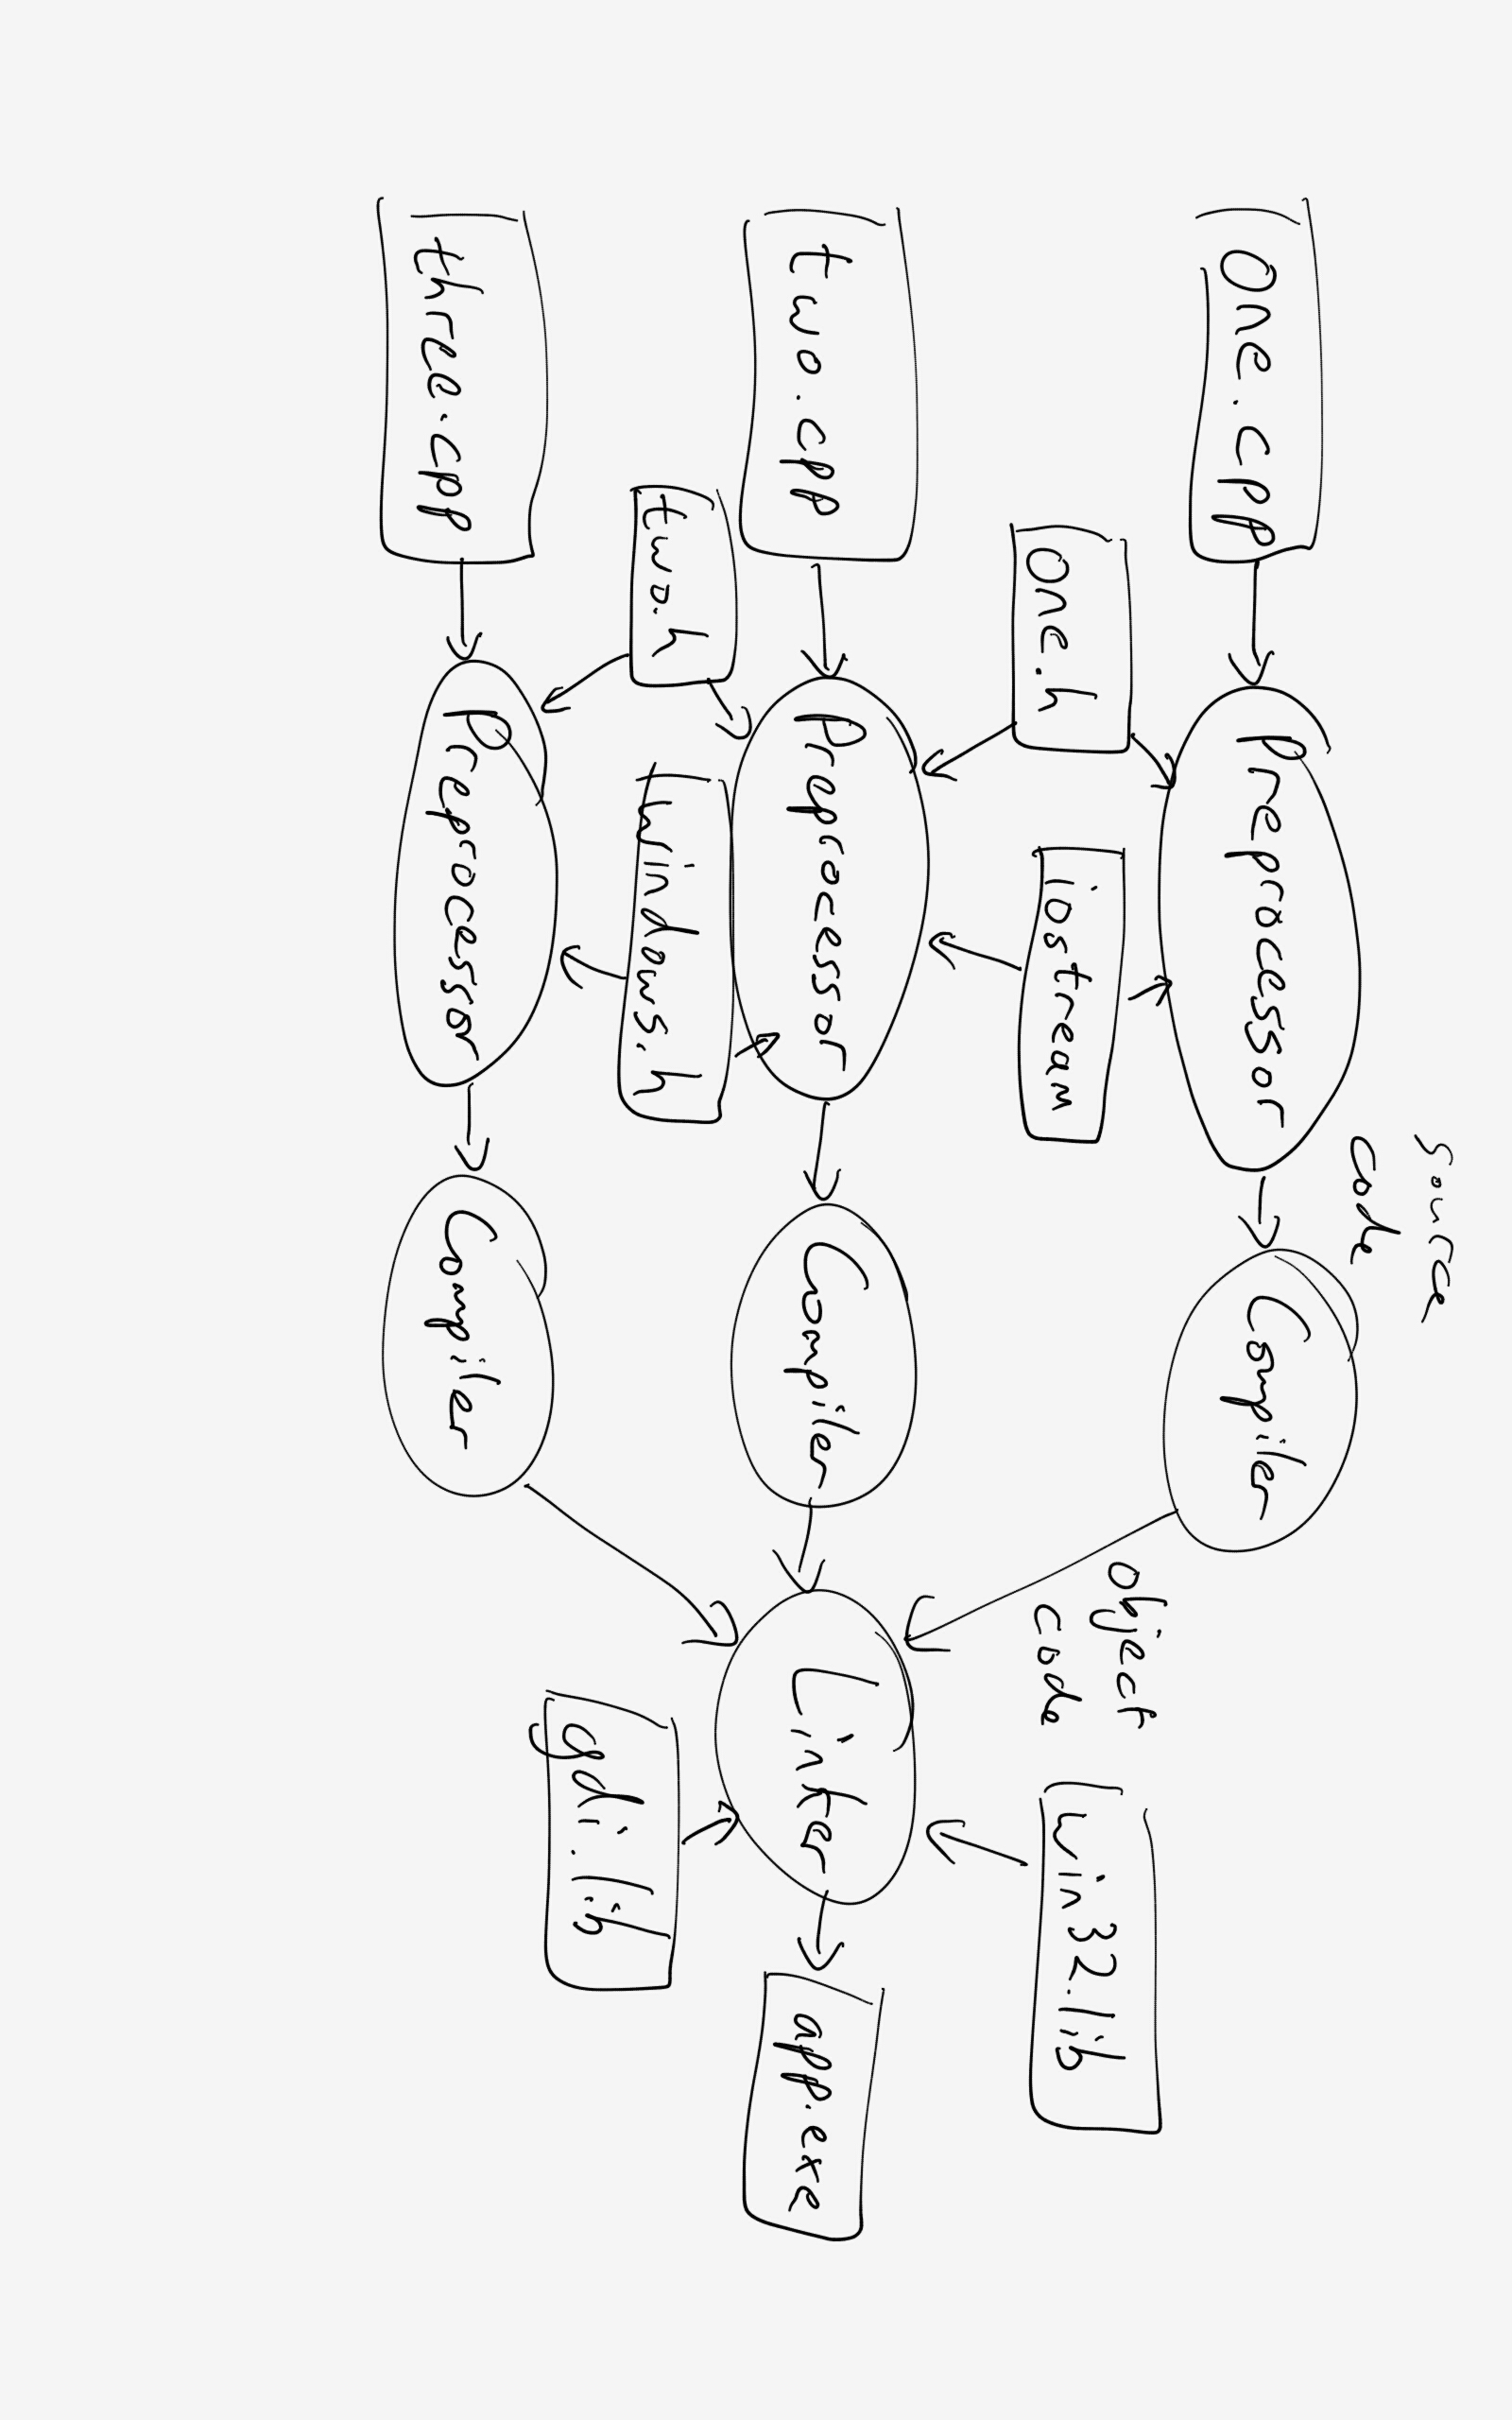
\includegraphics[height=\textwidth,angle=90]{compiler_sketch}
%\end{frame}

\end{document}
